\begin{spacing}{1.5}
\section{Overview}
The repository separates standalone classroom examples from configurable application implementations. The top-level Python lab files favor readable input, calculation and plotting steps. The app\_backend directory contains the registry, loader, validation, routes, shared helpers and parameterized operations. The Android project stages those sources with an offline adapter and builds a self-contained application [5,7].

\section{Technologies Used}
Desktop dependencies are specified as permitted version ranges in requirements.txt. Android uses a separate pinned package set because its embedded Python environment and binary libraries differ from desktop. Therefore, the two environments should not be described as sharing identical package versions. The report records declarations from the repository rather than treating those declarations as measured runtime versions.

\begin{table}[htbp]\centering\small
\caption{Declared platform technologies}
\begin{tabularx}{\textwidth}{XXX}
\toprule
\textbf{Component} & \textbf{Desktop declaration} & \textbf{Android declaration}\\\midrule
Python & Launcher targets Python 3.12 & Embedded Python 3.10\\
Interface & Flask 3.1 to below 4, HTML/CSS/JS & Native Java with Chaquopy 17.2.0\\
NumPy & 2.2 to below 3 & 1.23.3\\
OpenCV & Headless 4.11 to below 6 & 4.5.1.48\\
SciPy & 1.14 to below 2 & 1.8.1\\
Matplotlib & 3.9 to below 4 & 3.6.0\\
Pillow & 11 to below 13 & 9.2.0\\
Android platform & Not applicable & Minimum API 24, compile and target API 36\\
\bottomrule\end{tabularx}\end{table}
\section{Experiment and Course Preparation}
The catalog contains eight chapter records and 86 topic records. Chapter titles provide a navigation model, while topic records hold sources and presets. The morphology chapter has zero explicit topic records in the catalog even though the application includes a morphology operation. The desktop chapter fallback maps its operation group to chapter eight. Catalog topic counts must therefore be distinguished from executable chapter coverage [5].

The code tab displays a standalone default example, whereas the interactive controls call configurable backend functions. This distinction matters when reproducing a result: the current parameter settings must accompany the configurable implementation. Fixed-matrix experiments also continue to use the selected sample workflow for consistency, although their calculations depend on embedded course matrices rather than that sample [6].

\section{System Architecture}
On desktop, the browser handles image selection, controls and result presentation. Flask decodes inputs, retrieves the registry entry and calls the execution function. The backend returns image data and structured details for display. Plotting modules create figures and educational tables appropriate to the operation. The local launcher binds the experience to the user computer and opens the interface in a browser [5].

On Android, MainActivity provides image selection, chapter navigation, experiment controls and result display. The offline adapter invokes bundled Python operations directly through Chaquopy. No Flask process or local HTTP server is needed for this path. The manifest has no Internet permission, and the package includes arm64-v8a and x86\_64 libraries. API 24 is the minimum supported Android version in the Gradle configuration [7].

\begin{figure}[htbp]\centering
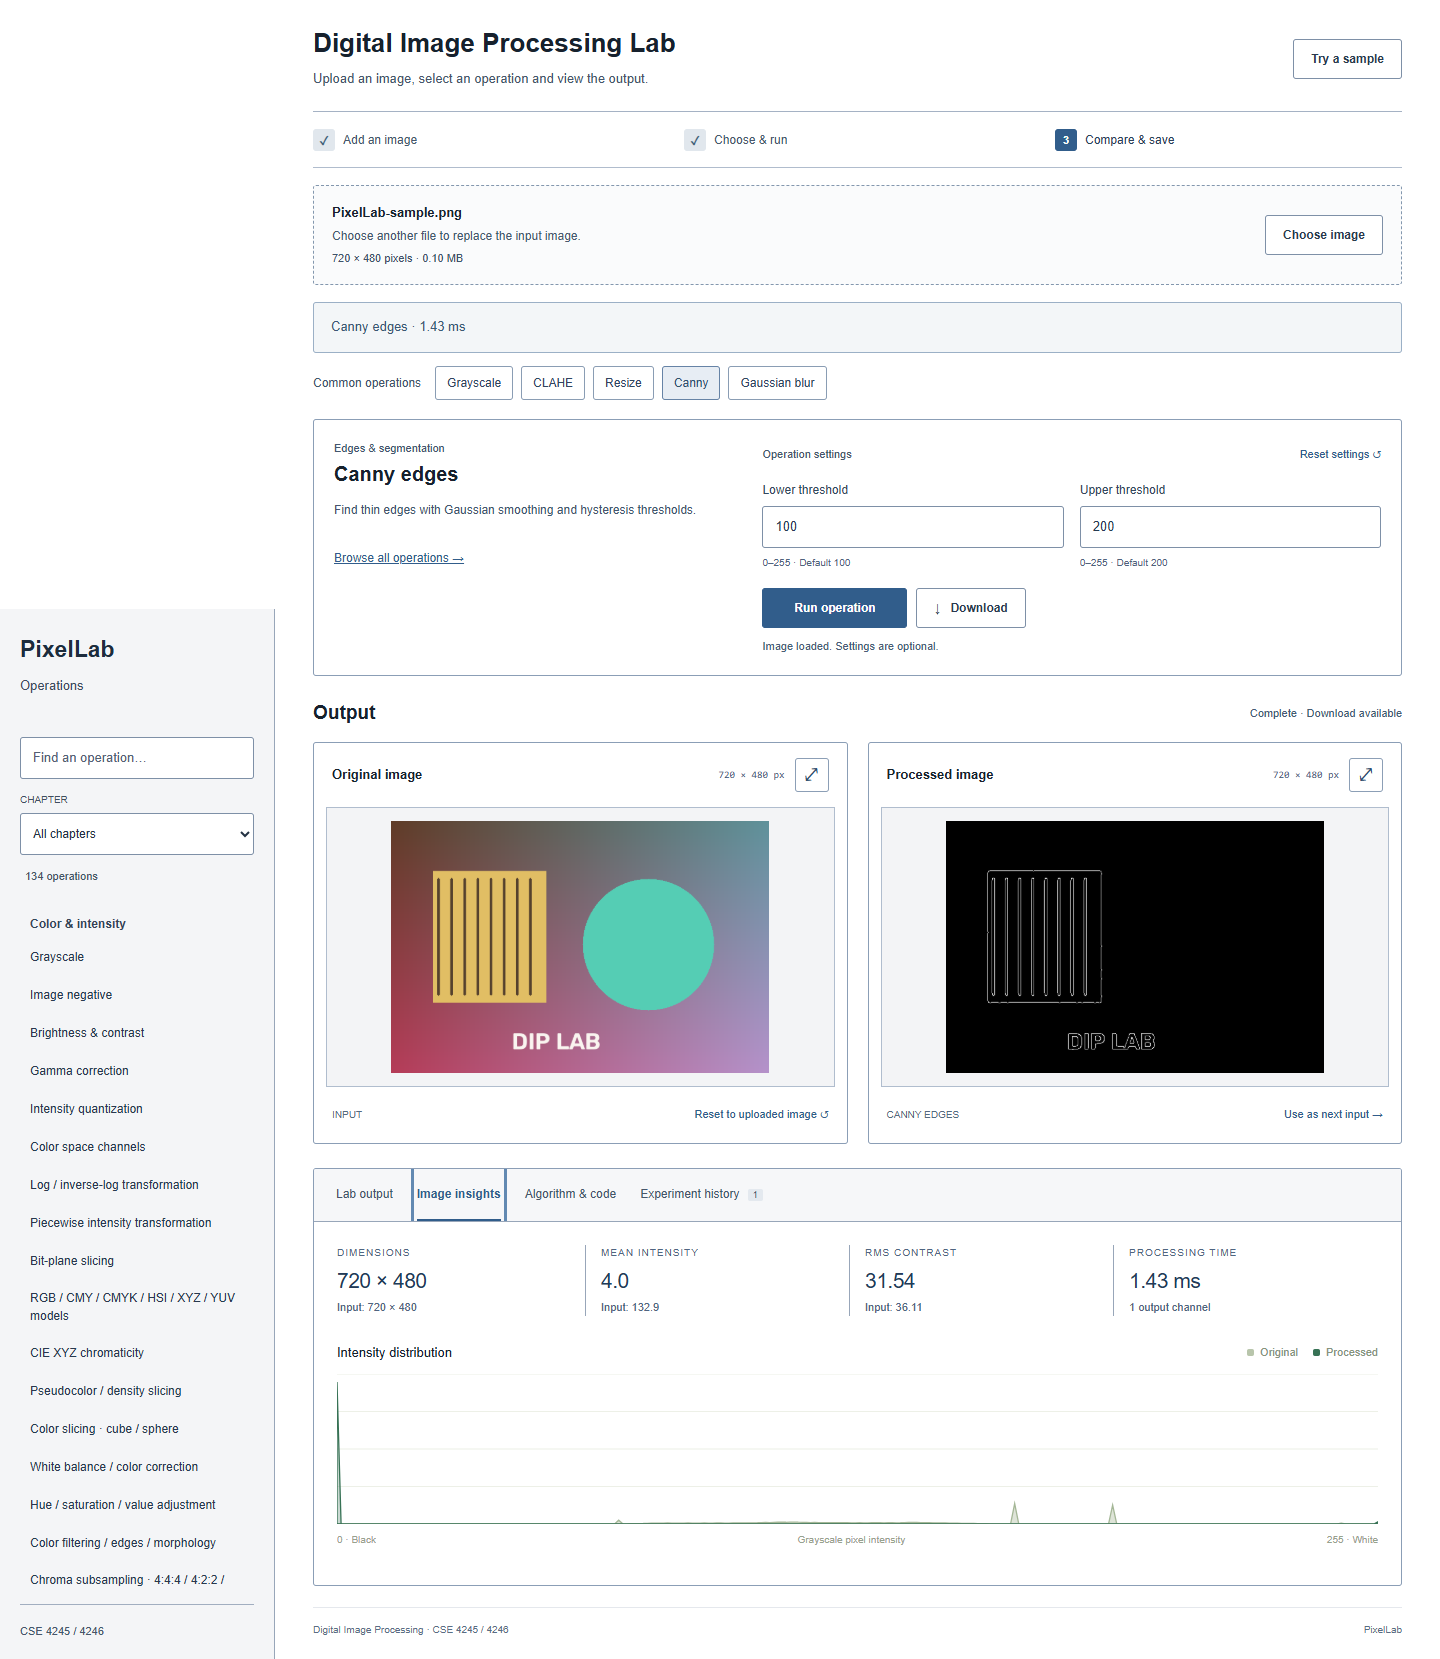
\includegraphics[width=5.8in,height=0.65\textheight,keepaspectratio]{Figures/friendly-desktop-result.png}
\caption{Retained desktop view of the PixelLab laboratory}
\end{figure}
\section{Implementation Details}
\subsection{Registry and Parameter Validation}
The operation decorator stores an identifier, display name, group, explanation, formula, source, field definitions and function reference. The loader imports modules to populate the registry. This provides one inventory for UI generation and execution checks. Grouped entries deliberately expose multiple variants, including noise models, morphology methods and lossless codecs [5].

The validator accepts only declared selection values, constrains text length and validates finite numeric values against field bounds. Integer fields reject fractional values. An even kernel is rejected rather than silently changed. These checks keep experiments reproducible and prevent controls from accepting values that conflict with backend assumptions.

\subsection{Plots Measurements and Export}
Operation-specific lab output is more informative than a uniform before-and-after chart. Geometry experiments report dimensions or crop regions, histogram experiments show distributions, transforms show spectra or reconstruction, and compression reports decoded output and encoded size. Grayscale histogram statistics are computed independently from the dedicated full-channel measurement option [5,6].

PNG saving preserves image pixels without lossy JPEG encoding. JPEG export contains actual JPEG bytes. The lossless JSON export includes dimensions, codec metadata and a base64 payload so that the teaching representation can be independently decoded. These artifacts have different purposes and should not be compared solely by their file extensions.

\subsection{Android Navigation and Packaging}
The Android sidebar contains chapter filters, combined chapter and text search, operation counts and a clear-filters action. Selecting an operation closes the drawer and preserves the input image. Back and the close control dismiss navigation. The package build stages current Python examples and the offline adapter, bundles dependencies, and signs the APK with the retained development key [7].

The delivered application version is declared as 2.2-offline with version code 4. The development signing configuration supports updates to earlier builds signed with that key, but a production release would need an appropriate release-signing and distribution process. Instrumented device-test builds are separate from the APK intended for ordinary installation.

\begin{figure}[htbp]\centering
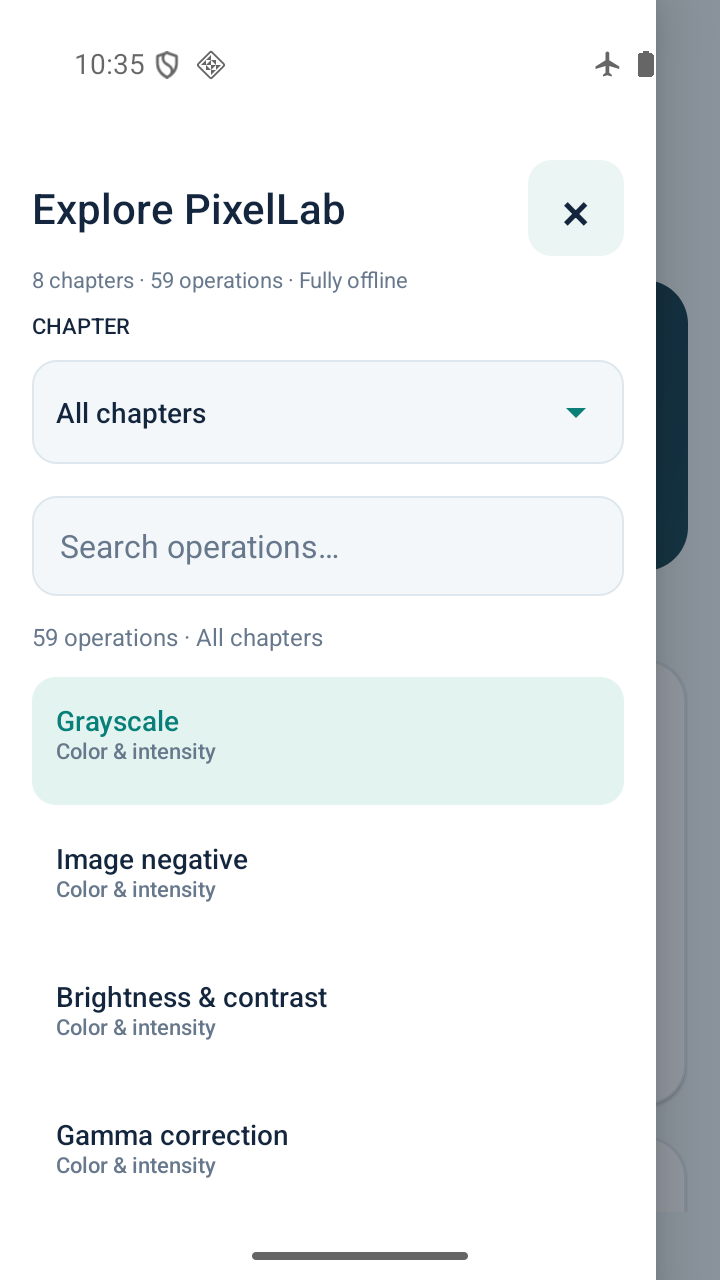
\includegraphics[width=2.8in,height=0.65\textheight,keepaspectratio]{Figures/sidebar-open.png}
\caption{Retained Android sidebar showing chapter and operation navigation}
\end{figure}
\end{spacing}